Per poter assicurare una conduzione e uno sviluppo del progetto che soddisfino le scadenze riportate nella sezione xxx, il gruppo ha deciso di ripartire il lasso di tempo che va dalla sua formazione fino alla revisione di accettazione nelle seguenti cinque attività:
	
	\begin{itemize}
		\item Analisi dei requisiti
		\item Consolidamento dei requisiti
		\item Progettazione della technology baseline
		\item Progettazione di dettaglio e codifica
		\item Validazione e collaudo
	\end{itemize}
	
	Ogni attività verrà poi frammentata in altri sottoperiodi, in ognuno dei quali verrà associata una \glock{Milestone},
	riferita alla data di fine periodo, per il completamento delle singole attività previste al suo interno.
	In intervallo di tempo vengono quindi inserite più attività, le quali possono essere svolte sia sequenzialmente,
	sia con un certo grado di parallelismo, in base alle dipendenze che sussistono tra di loro.
	
	\subsection{Analisi dei Requisiti}
	L’attività di analisi dei requisiti ha inizio il giorno 31-10-2021, successivamente alla formazione dei
	gruppi, ed è suddivisa in cinque periodi, con termine fissato per il giorno 11-01-2021, giorno di consegna dei documenti in ingresso alla revisione dei requisiti.
	
	\subsection{Ruoli attivi}
	Durante questa attività è necessaria la presenza dei seguenti ruoli:
	\begin{itemize}
		\item responsabile;
		\item amministratore;
		\item analista;
		\item verificatore;
	\end{itemize}

	\subsection{Periodi}
	L’attività di analisi dei requisiti è stata suddivisa nei seguenti cinque periodi:
	
	\subsubsection{Primo periodo dal 31-10-2021 al 05-12-2021}
	\begin{itemize}
	\item \textbf{Analisi dei capitolati}: studio individuale dei capitolati e discussione interna al gruppo dei pregi e svantaggi individuati da ogni componente, in modo da indirizzare l’interesse del gruppo su certi capitolati piuttosto che su altri;
	\item \textbf{Ricerca}: individuazione e studio degli strumenti e delle tecnologie di supporto da utilizzare per
	la gestione del progetto;
	\item \textbf{Studio di fattibilità}: impostato sulla base dell’analisi dei capitolati fatta in precedenza;
	\item \textbf {Pianificazione attività}: decisione dell’organizzazione interna al gruppo riguardo i ruoli
	da assegnare ed i compiti da svolgere.
	\end{itemize}
	
	\subsubsection{Secondo periodo dal 05-12-2021 al 17-12-2021}
	\begin{itemize}
	\item \textbf{Scelta del capitolato}: decisione definitiva riguardo il capitolato scelto;
	\item \textbf{Normazione}: scelta delle regole da adottare durante lo sviluppo del progetto riguardanti i
	processi primari e processi organizzativi;
	\item \textbf{Studio di fattibilità}: fine dello studio di fattibilità, basato sul capitolato scelto;
	\end{itemize}
	
	\subsubsection{Terzo periodo dal 18-12-2021 al 29-12-2021}
	\begin{itemize}
		\item \textbf{Analisi dei casi d'uso}: analisi del prodotto e dei casi d’uso;
		\item \textbf{Norme di progetto}: stesura delle norme di progetto;
		\item \textbf{Piano di progetto}: stesura del piano di progetto;
		\item \textbf{Analisi dei rischi}: individuazione dei rischi che possono presentarsi nello svolgimento del
		progetto.
	\end{itemize}
	
	\subsubsection{Quarto periodo dal 30-12-2021 al 07-01-2021}
	\begin{itemize}
	\item \textbf{Analisi dei requisiti}: analisi dei requisiti e tracciamento;
	\item \textbf{Piano di qualifica}: stesura del piano di qualifica;
	\item \textbf{Glossario}: stesura del glossario.
	\end{itemize}
	
	\subsubsection{Quinto periodo dal 08-01-2021 al 11-01-2021}
	\begin{itemize}
	\item \textbf{Revisione}: ultimo controllo di tutti i documenti scritti;
	\item \textbf{Presentazione RR}: presentazione della revisione dei requisiti.
	\end{itemize}
	
	
	\newpage
	
%	\KOMAoptions{paper=landscape,pagesize}
%	\begin{figure}[h!]
%	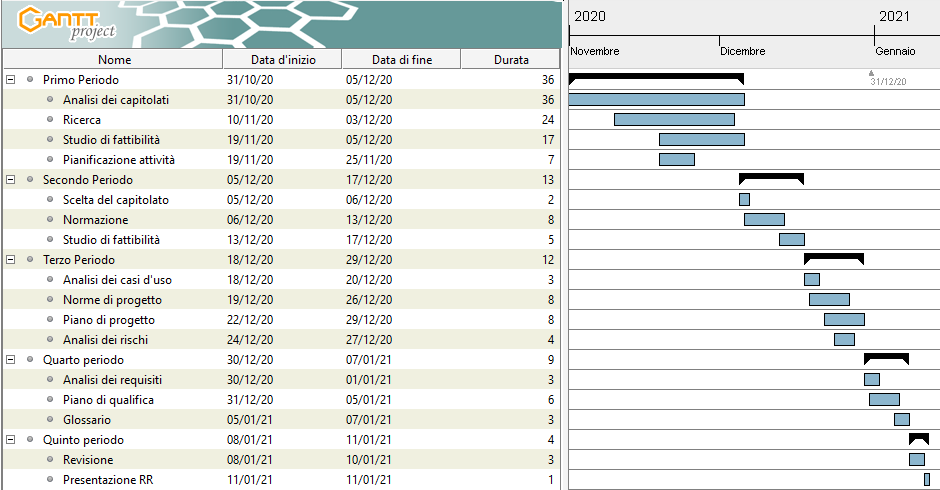
\includegraphics[width=1.7\textwidth]{images/1_Analisi_dei_requisiti.png}
%	\caption{Analisi dei requisiti}
%	\end{figure}
	
	\newpage
%	\KOMAoptions{paper=portrait,pagesize}
	
	\subsection{Consolidamento dei Requisiti}
	L’attività di consolidamento dei requisiti ha inizio il giorno 12-01-2021, successivamente alla consegna
	del materiale in ingresso alla revisione dei requisiti, ed è suddivisa in due periodi, con termine fissato
	per il giorno 17-01-2021, che precede la revisione dei requisiti del 18-01-2021.
	
	\subsection{Ruoli attivi}
	Durante questa attività è necessaria la presenza dei seguenti ruoli:
	\begin{itemize}
	\item responsabile;
	\item amministratore;
	\item analista.
	\end{itemize}

	\subsection{Periodi}
	L’attività di consolidamento dei requisiti è stata suddivisa nei seguenti due periodi:
	
	\subsubsection{Primo periodo dal 12-01-2021 al 15-01-2021}
	\begin{itemize}
	
	\item \textbf{Preparazione presentazione}: redazione della presentazione da portare in sede di revisione e
	studio individuale.
	
	\end{itemize}	
	
	\subsubsection{Secondo periodo dal 16-01-2021 al 17-01-2021}
	\begin{itemize}
		
	\item \textbf{Analisi dei requisiti}: revisione ed eventuale aggiornamento dei requisiti.
		
	\end{itemize}

	\newpage
	
%	\KOMAoptions{paper=landscape,pagesize}
%	\begin{figure}[h!]
%	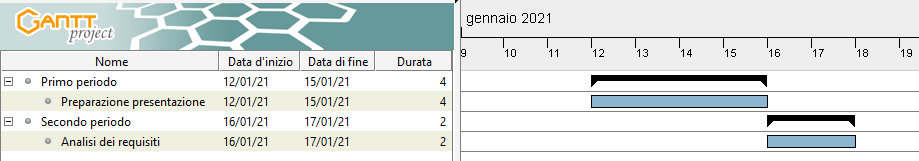
\includegraphics[width=1.7\textwidth]{images/2_Consolidamento_dei_requisiti.png}
%	\caption{Consolidamento dei requisiti}
%	\end{figure}

	\newpage
%	\KOMAoptions{paper=portrait,pagesize}

	
	\subsection{Progettazione della Technology Baseline}
	L’attività di progettazione della technology baseline ha inizio il giorno 19-01-2021, successivamente
	alla revisione dei requisiti, ed è suddivisa in tre periodi, con termine fissato per il giorno 07-01-2021,
	che precede la revisione di progettazione del 08-03-2021.
	
	\subsubsection{Ruoli attivi}
	Durante questa attività è necessaria la presenza dei seguenti ruoli:
	\begin{itemize}
	\item responsabile;
	\item amministratore;
	\item analista;
	\item progettista;
	\item programmatore;
	\item verificatore;
	\end{itemize}

	\subsubsection{Periodi}
	L’attività di progettazione della technology baseline è stata suddivisa nei seguenti periodi:
	
	\subsubsection{Primo periodo dal 19-01-2021 al 11-02-2021}
	\begin{itemize}
	\item \textbf{Normazione}: revisione ed eventuale aggiornamento delle norme;
	\item \textbf{Aggiornamento della pianificazione};
	\item \textbf{Aggiornamento della qualità};
	\item {Analisi dei requisiti}: revisione ed eventuale aggiornamento dei casi d’uso e dei requisiti, in base
	alle indicazioni ricevute;
	\item \textbf{Ricerca}: studio autonomo degli strumenti e le tecnologie da utilizzare per lo sviluppo del
	progetto;
	\item \textbf{Progettazione};
	\item \textbf{Verifica}: controllo della qualità di tutti i prodotti sviluppati durante il periodo attuale.
	\end{itemize}

	\subsubsection{Secondo periodo dal 12-02-2021 al 03-03-2021}
	\begin{itemize}
	\item \textbf{Normazione}: aggiornamento delle norme;
	\item \textbf{Progettazione}: progettazione del PROOF OF CONCEPTG che deve essere implementato;
	\item \textbf{Aggiornamento della pianificazione};
	\item \textbf{Codifica}: implementazione del PROOF OF CONCEPTG progettato;
	\item \textbf{Stesura della lettera di presentazione}: scrittura della lettera di presentazione con la quale ci
	si candida alla revisione di progettazione;
	\item \textbf{Verifica}: controllo della qualità di tutti i prodotti sviluppati durante il periodo attuale.
	\end{itemize}	
	
	\subsubsection{Terzo periodo dal 04-03-2021 al 07-03-2021}
	\begin{itemize}
	\item \textbf{Preparazione presentazione}: redazione della presentazione da portare in sede di revisione e
	studio individuale.
	\end{itemize}

	\begin{landscape}
	\newpage
	
	\begin{figure}[h!]
	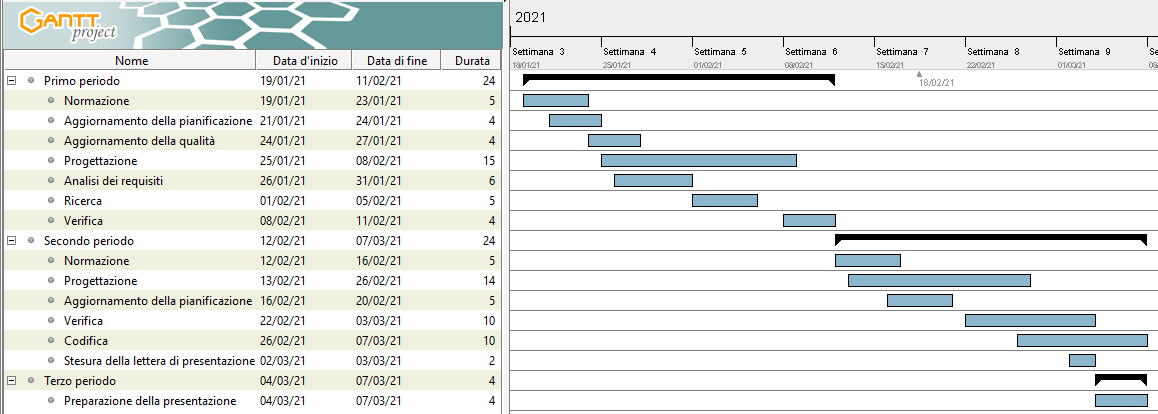
\includegraphics[width=1.7\textwidth]{images/3_Progettazione_della_Technology.png}
	\caption{Progettazione della Technology}
	\end{figure}
	\end{landscape}
	
	\newpage	
	
	\subsection{Progettazione di dettaglio e Codifica}
	L’attività di progettazione di dettaglio e codifica ha inizio il giorno 09-03-2021, successivamente alla
	revisione di progettazione, ed è suddivisa in tre periodi, con termine fissato per il giorno 08-04-2021,
	che precede la revisione di qualifica del 09-04-2021.
	
	\subsubsection{Ruoli attivi}
	Durante questa attività è necessaria la presenza dei seguenti ruoli:
	\begin{itemize}
	\item responsabile;
	\item amministratore;
	\item progettista;
	\item programmatore;
	\item verificatore;
	\end{itemize}

	\subsubsection{Periodi}
	L’attività di progettazione di dettaglio e codifica è stata suddivisa nei seguenti periodi:
	\subsubsection{Primo periodo dal 09-03-2021 al 18-03-2021}
	\begin{itemize}
		\item \textbf{Normazione}: aggiornamento delle norme;
		\item \textbf{Aggiornamento della pianificazione};
		\item \textbf{Aggiornamento della qualità};
		\item \textbf{Progettazione}: miglioramento incrementale della progettazione fatta per il PROOF OF CONCEPTG;
		\item \textbf{Codifica}: implementazione prodotto software e test;
		\item \textbf{Scrittura manuale}: prima stesura;
		\item \textbf{Verifica}: controllo della qualità di tutti i prodotti sviluppati durante il periodo attuale.
	\end{itemize}

	\subsubsection{Secondo periodo dal 19-03-2021 al 30-03-2021}
	\begin{itemize}
	\item \textbf{Normazione}: aggiornamento delle norme;
	\item \textbf{Aggiornamento della pianificazione};
	\item \textbf{Progettazione}: miglioramento incrementale della progettazione tramite DESIGN PATTERNG;
	\item \textbf{Codifica}: primo rilascio;
	\item \textbf{Aggiornamento manuale};
	\item \textbf{Stesura della lettera di presentazione}: scrittura della lettera di presentazione con la quale ci
	si candida alla revisione di qualifica;
	\item \textbf{Verifica}: controllo della qualità di tutti i prodotti sviluppati durante il periodo attuale.
	\end{itemize}

	\subsubsection{Terzo periodo dal 31-03-2021 al 08-04-2021}
	\begin{itemize}
	\item \textbf{Preparazione presentazione}: redazione della presentazione da portare in sede di revisione e
	studio individuale.
	\end{itemize}

	\newpage
%	\KOMAoptions{paper=landscape,pagesize}
%	\begin{figure}[h!]
%	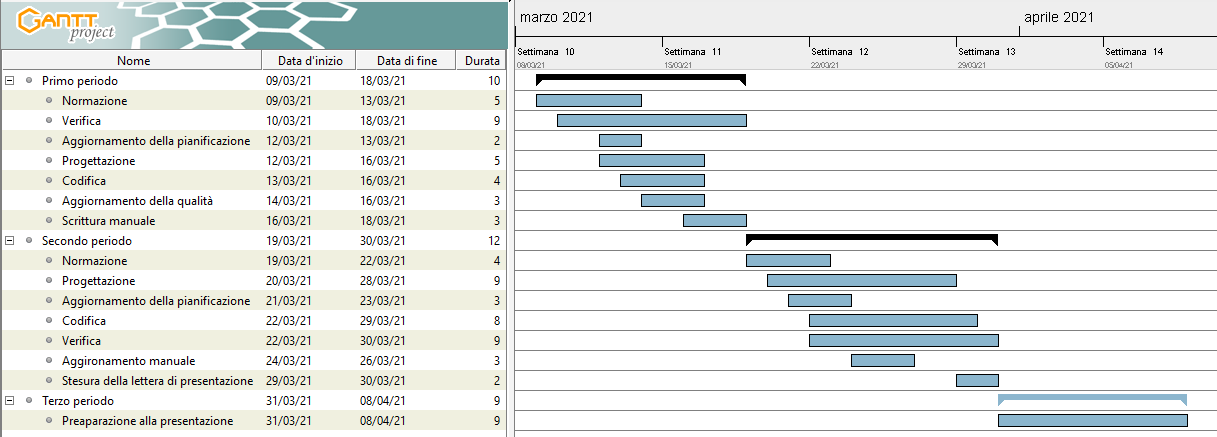
\includegraphics[width=1.7\textwidth]{images/4_Progettazione_e_codifica.png}
%	\caption{Progettazione e codifica}
%	\end{figure}
	
	\newpage
%	\KOMAoptions{paper=portrait,pagesize}
	
	\newpage

	\subsection{Validazione e Collaudo}
	L’attività di validazione e collaudo ha inizio il giorno 10-04-2021, successivamente alla revisione di
	qualifica, ed è suddivisa in tre periodi, con termine fissato per il giorno 09-05-2021, che precede la
	revisione di accettazione del 10-05-2021.
	
	\subsubsection{Ruoli attivi}
	Durante questa attività è necessaria la presenza dei seguenti ruoli:
	\begin{itemize}
		\item responsabile;
		\item amministratore;
		\item progettista;
		\item programmatore;
		\item verificatore;
	\end{itemize}

	\subsubsection{Periodi}
	L’attività di validazione e collaudo è stata suddivisa nei seguenti periodi:
	\subsubsection{Primo periodo dal 10-04-2021 al 23-04-2021}
	\begin{itemize}
		\item \textbf{Normazione}: revisione ed eventuale aggiornamento delle norme;
		\item \textbf{Aggiornamento} della pianificazione;
		\item \textbf{Aggiornamento della qualità};
		\item \textbf{Completamento progettazione};
		\item \textbf{Verifica}: controllo della qualità di tutti i prodotti sviluppati durante il periodo attuale.
	\end{itemize}

	\subsubsection{Secondo periodo dal 24-04-2021 al 02-05-2021}
	\begin{itemize}
		\item \textbf{Codifica}: rilascio ultima versione;
		\item \textbf{Completamento manuale};
		\item \textbf{Verifica}: controllo della qualità di tutti i prodotti sviluppati durante il periodo attuale, in
		particolare sono eseguiti i test per la verifica del software.
	\end{itemize}

	\subsubsection{Terzo periodo dal 03-05-2021 al 09-05-2021}
	\begin{itemize}
		\item \textbf{Preparazione presentazione}: redazione della presentazione da portare in sede di revisione e
		studio individuale.
	\end{itemize}

	\newpage
%	\KOMAoptions{paper=landscape,pagesize}
%	\begin{figure}[h!]
%	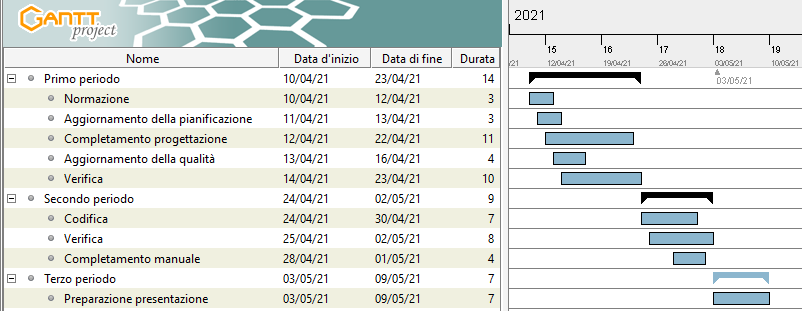
\includegraphics[width=1.7\textwidth]{images/5_Validazione_e_collaudo.png}
%	\caption{Validazione e collaudo}
%	\end{figure}
	
	\newpage
%	\KOMAoptions{paper=portrait,pagesize}